%\documentclass{article}

%\usepackage{amssymb, amsfonts,amsthm,amsmath}
%\usepackage{enumitem}
%\usepackage{hyperref,xcolor}

%\def\inputGnumericTable{}
%\usepackage{array}
%\usepackage{longtable}
%\usepackage{calc}
%\usepackage{multirow}
%\usepackage{hhline}
%\usepackage{ifthen}



%\begin{document}
%\title{Details of the NavIC frequency bands }
%\author{\Large Shreyash Putta - FWC22070}
%\date{}

%\maketitle

%\section{NavIC frequency bands}
\section{The Frequency Bands}
An independent Indian Satellite based positioning system for critical National applications. The main objective is to provide Reliable Position, Navigation and Timing services over India and its neighbourhood, to provide fairly good accuracy to the user. 

	
	\begin{table}[h!]
	\small
	\centering
	\caption{the navic frequency bands}
	\label{table:bands}
	%\subimport{table/}{table1.tex}
	%%%%%%%%%%%%%%%%%%%%%%%%%%%%%%%%%%%%%%%%%%%%%%%%%%%%%%%%%%%%%%%%%%%%%%
%%                                                                  %%
%%  This is the header of a LaTeX2e file exported from Gnumeric.    %%
%%                                                                  %%
%%  This file can be compiled as it stands or included in another   %%
%%  LaTeX document. The table is based on the longtable package so  %%
%%  the longtable options (headers, footers...) can be set in the   %%
%%  preamble section below (see PRAMBLE).                           %%
%%                                                                  %%
%%  To include the file in another, the following two lines must be %%
%%  in the including file:                                          %%
%%        \def\inputGnumericTable{}                                 %%
%%  at the beginning of the file and:                               %%
%%        \input{name-of-this-file.tex}                             %%
%%  where the table is to be placed. Note also that the including   %%
%%  file must use the following packages for the table to be        %%
%%  rendered correctly:                                             %%
%%    \usepackage[latin1]{inputenc}                                 %%
%%    \usepackage{color}                                            %%
%%    \usepackage{array}                                            %%
%%    \usepackage{longtable}                                        %%
%%    \usepackage{calc}                                             %%
%%    \usepackage{multirow}                                         %%
%%    \usepackage{hhline}                                           %%
%%    \usepackage{ifthen}                                           %%
%%  optionally (for landscape tables embedded in another document): %%
%%    \usepackage{lscape}                                           %%
%%                                                                  %%
%%%%%%%%%%%%%%%%%%%%%%%%%%%%%%%%%%%%%%%%%%%%%%%%%%%%%%%%%%%%%%%%%%%%%%



%%  This section checks if we are begin input into another file or  %%
%%  the file will be compiled alone. First use a macro taken from   %%
%%  the TeXbook ex 7.7 (suggestion of Han-Wen Nienhuys).            %%
\def\ifundefined#1{\expandafter\ifx\csname#1\endcsname\relax}


%%  Check for the \def token for inputed files. If it is not        %%
%%  defined, the file will be processed as a standalone and the     %%
%%  preamble will be used.                                          %%
\ifundefined{inputGnumericTable}

%%  We must be able to close or not the document at the end.        %%
	\def\gnumericTableEnd{\end{document}}


%%%%%%%%%%%%%%%%%%%%%%%%%%%%%%%%%%%%%%%%%%%%%%%%%%%%%%%%%%%%%%%%%%%%%%
%%                                                                  %%
%%  This is the PREAMBLE. Change these values to get the right      %%
%%  paper size and other niceties.                                  %%
%%                                                                  %%
%%%%%%%%%%%%%%%%%%%%%%%%%%%%%%%%%%%%%%%%%%%%%%%%%%%%%%%%%%%%%%%%%%%%%%

	\documentclass[12pt%
			  %,landscape%
                    ]{report}
       \usepackage[latin1]{inputenc}
       \usepackage{fullpage}
       \usepackage{color}
       \usepackage{array}
       \usepackage{longtable}
       \usepackage{calc}
       \usepackage{multirow}
       \usepackage{hhline}
       \usepackage{ifthen}

	\begin{document}


%%  End of the preamble for the standalone. The next section is for %%
%%  documents which are included into other LaTeX2e files.          %%
\else

%%  We are not a stand alone document. For a regular table, we will %%
%%  have no preamble and only define the closing to mean nothing.   %%
    \def\gnumericTableEnd{}

%%  If we want landscape mode in an embedded document, comment out  %%
%%  the line above and uncomment the two below. The table will      %%
%%  begin on a new page and run in landscape mode.                  %%
%       \def\gnumericTableEnd{\end{landscape}}
%       \begin{landscape}


%%  End of the else clause for this file being \input.              %%
\fi

%%%%%%%%%%%%%%%%%%%%%%%%%%%%%%%%%%%%%%%%%%%%%%%%%%%%%%%%%%%%%%%%%%%%%%
%%                                                                  %%
%%  The rest is the gnumeric table, except for the closing          %%
%%  statement. Changes below will alter the table's appearance.     %%
%%                                                                  %%
%%%%%%%%%%%%%%%%%%%%%%%%%%%%%%%%%%%%%%%%%%%%%%%%%%%%%%%%%%%%%%%%%%%%%%

\providecommand{\gnumericmathit}[1]{#1} 
%%  Uncomment the next line if you would like your numbers to be in %%
%%  italics if they are italizised in the gnumeric table.           %%
%\renewcommand{\gnumericmathit}[1]{\mathit{#1}}
\providecommand{\gnumericPB}[1]%
{\let\gnumericTemp=\\#1\let\\=\gnumericTemp\hspace{0pt}}
 \ifundefined{gnumericTableWidthDefined}
        \newlength{\gnumericTableWidth}
        \newlength{\gnumericTableWidthComplete}
        \newlength{\gnumericMultiRowLength}
        \global\def\gnumericTableWidthDefined{}
 \fi
%% The following setting protects this code from babel shorthands.  %%
 \ifthenelse{\isundefined{\languageshorthands}}{}{\languageshorthands{english}}
%%  The default table format retains the relative column widths of  %%
%%  gnumeric. They can easily be changed to c, r or l. In that case %%
%%  you may want to comment out the next line and uncomment the one %%
%%  thereafter                                                      %%
\providecommand\gnumbox{\makebox[0pt]}
%%\providecommand\gnumbox[1][]{\makebox}

%% to adjust positions in multirow situations                       %%
\setlength{\bigstrutjot}{\jot}
\setlength{\extrarowheight}{\doublerulesep}

%%  The \setlongtables command keeps column widths the same across  %%
%%  pages. Simply comment out next line for varying column widths.  %%
\setlongtables

\setlength\gnumericTableWidth{%
	53pt+%
	107pt+%
	65pt+%
	65pt+%
0pt}
\def\gumericNumCols{3}
\setlength\gnumericTableWidthComplete{\gnumericTableWidth+%
         \tabcolsep*\gumericNumCols*2+\arrayrulewidth*\gumericNumCols}
\ifthenelse{\lengthtest{\gnumericTableWidthComplete > \linewidth}}%
         {\def\gnumericScale{\ratio{\linewidth-%
                        \tabcolsep*\gumericNumCols*2-%
                        \arrayrulewidth*\gumericNumCols}%
{\gnumericTableWidth}}}%
{\def\gnumericScale{1}}

%%%%%%%%%%%%%%%%%%%%%%%%%%%%%%%%%%%%%%%%%%%%%%%%%%%%%%%%%%%%%%%%%%%%%%
%%                                                                  %%
%% The following are the widths of the various columns. We are      %%
%% defining them here because then they are easier to change.       %%
%% Depending on the cell formats we may use them more than once.    %%
%%                                                                  %%
%%%%%%%%%%%%%%%%%%%%%%%%%%%%%%%%%%%%%%%%%%%%%%%%%%%%%%%%%%%%%%%%%%%%%%

\ifthenelse{\isundefined{\gnumericColA}}{\newlength{\gnumericColA}}{}\settowidth{\gnumericColA}{\begin{tabular}{@{}p{40pt*\gnumericScale}@{}}x\end{tabular}}
\ifthenelse{\isundefined{\gnumericColB}}{\newlength{\gnumericColB}}{}\settowidth{\gnumericColB}{\begin{tabular}{@{}p{85pt*\gnumericScale}@{}}x\end{tabular}}
\ifthenelse{\isundefined{\gnumericColC}}{\newlength{\gnumericColC}}{}\settowidth{\gnumericColC}{\begin{tabular}{@{}p{60pt*\gnumericScale}@{}}x\end{tabular}}
\ifthenelse{\isundefined{\gnumericColD}}{\newlength{\gnumericColD}}{}\settowidth{\gnumericColD}{\begin{tabular}{@{}p{112pt*\gnumericScale}@{}}x\end{tabular}}
\begin{longtable}[c]{%
	b{\gnumericColA}%
	b{\gnumericColB}%
	b{\gnumericColC}%
	b{\gnumericColD}%
	}

%%%%%%%%%%%%%%%%%%%%%%%%%%%%%%%%%%%%%%%%%%%%%%%%%%%%%%%%%%%%%%%%%%%%%%
%%  The longtable options. (Caption, headers... see Goosens, p.124) %%
%	\caption{The Table Caption.}             \\	%
% \hline	% Across the top of the table.
%%  The rest of these options are table rows which are placed on    %%
%%  the first, last or every page. Use \multicolumn if you want.    %%

%%  Header for the first page.                                      %%
%	\multicolumn{3}{c}{The First Header} \\ \hline 
%	\multicolumn{1}{c}{colTag}	%Column 1
%	&\multicolumn{1}{c}{colTag}	%Column 2
%	&\multicolumn{1}{c}{colTag}	\\ \hline %Last column
%	\endfirsthead

%%  The running header definition.                                  %%
%	\hline
%	\multicolumn{3}{l}{\ldots\small\slshape continued} \\ \hline
%	\multicolumn{1}{c}{colTag}	%Column 1
%	&\multicolumn{1}{c}{colTag}	%Column 2
%	&\multicolumn{1}{c}{colTag}	\\ \hline %Last column
%	\endhead

%%  The running footer definition.                                  %%
%	\hline
%	\multicolumn{3}{r}{\small\slshape continued\ldots} \\
%	\endfoot

%%  The ending footer definition.                                   %%
%	\multicolumn{3}{c}{That's all folks} \\ \hline 
%	\endlastfoot
%%%%%%%%%%%%%%%%%%%%%%%%%%%%%%%%%%%%%%%%%%%%%%%%%%%%%%%%%%%%%%%%%%%%%%

\hhline{|-|-|-|-}
	 \multicolumn{1}{|p{\gnumericColA}|}%
	{\gnumericPB{\raggedright}\gnumbox[l]{Bands}}
	&\multicolumn{1}{p{\gnumericColB}|}%
	{\gnumericPB{\raggedright}\gnumbox[l]{Carrier Frequency}}
	&\multicolumn{1}{p{\gnumericColC}|}%
	{\gnumericPB{\raggedright}\gnumbox[l]{Bandwidth}}
	&\multicolumn{1}{p{\gnumericColD}|}%
	{\gnumericPB{\raggedright}\gnumbox[l]{Usage}}
\\
\hhline{|----|}
	 \multicolumn{1}{|p{\gnumericColA}|}%
	{\gnumericPB{\raggedright}\gnumbox[l]{L1}}
	&\multicolumn{1}{p{\gnumericColB}|}%
	{\gnumericPB{\raggedright}\gnumbox[l]{1575.42 Mhz}}
	&\multicolumn{1}{p{\gnumericColC}|}%
	{\gnumericPB{\raggedright}\gnumbox[l]{24 Mhz}}
	&\multicolumn{1}{p{\gnumericColD}|}%
	{\gnumericPB{\raggedright}\gnumbox[l]{for low power devices}}
\\
\hhline{|----|}
	 \multicolumn{1}{|p{\gnumericColA}|}%
	{\gnumericPB{\raggedright}\gnumbox[l]{L5}}
	&\multicolumn{1}{p{\gnumericColB}|}%
	{\gnumericPB{\raggedright}\gnumbox[l]{1176.45 Mhz}}
	&\multicolumn{1}{p{\gnumericColC}|}%
	{\gnumericPB{\raggedright}\gnumbox[l]{24 Mhz}}
	&\multicolumn{1}{p{\gnumericColD}|}%
	{\gnumericPB{\raggedright}\gnumbox[l]{navigation and positioning}}
\\
\hhline{|----|}
	 \multicolumn{1}{|p{\gnumericColA}|}%
	{\gnumericPB{\raggedright}\gnumbox[l]{S}}
	&\multicolumn{1}{p{\gnumericColB}|}%
	{\gnumericPB{\raggedright}\gnumbox[l]{2492.028 Mhz}}
	&\multicolumn{1}{p{\gnumericColC}|}%
	{\gnumericPB{\raggedright}\gnumbox[l]{16.5 Mhz}}
	&\multicolumn{1}{p{\gnumericColD}|}%
	{\gnumericPB{\raggedright}\gnumbox[l]{SBAS and messaging}}

\\
\hhline{|-|-|-|-|}
\end{longtable}

\ifthenelse{\isundefined{\languageshorthands}}{}{\languageshorthands{\languagename}}
\gnumericTableEnd

	\end{table}

%make a table to this data
Because of satellites’ increased use, number and size, congestion has become a serious issue in the lower frequency bands
	\begin{figure}[h!]
	\centering
	\tikzset{every picture/.style={line width=0.75pt}} %set default line width to 0.75pt        
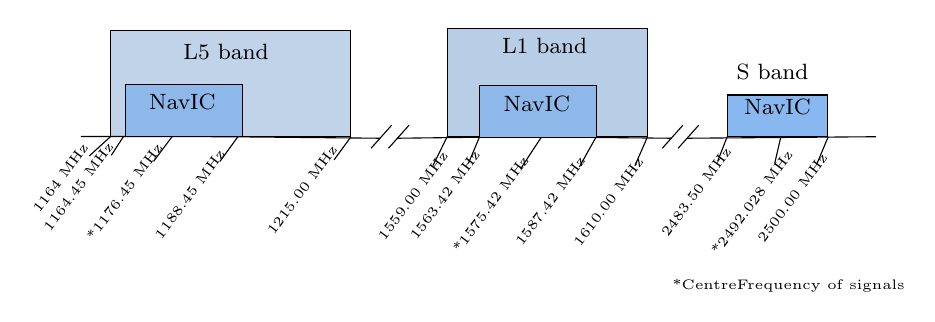
\begin{tikzpicture}[x=0.75pt,y=0.75pt,yscale=-1,xscale=1]
%uncomment if require: \path (0,471); %set diagram left start at 0, and has height of 471

%Shape: Rectangle [id:dp9517205987034671] 
\draw  [fill={rgb, 255:red, 192; green, 211; blue, 233 }  ,fill opacity=1 ] (92.53,176.6) -- (208.12,176.6) -- (208.12,227.79) -- (92.53,227.79) -- cycle ;
%Shape: Rectangle [id:dp3424557357689655] 
\draw  [fill={rgb, 255:red, 184; green, 205; blue, 230 }  ,fill opacity=1 ] (254.8,175.52) -- (351.33,175.52) -- (351.33,227.79) -- (254.8,227.79) -- cycle ;
%Shape: Rectangle [id:dp8560354037740456] 
\draw  [fill={rgb, 255:red, 137; green, 183; blue, 239 }  ,fill opacity=1 ] (389.7,207.67) -- (438,207.67) -- (438,227.79) -- (389.7,227.79) -- cycle ;
%Straight Lines [id:da4982550625943454] 
\draw    (78.33,227.67) -- (148.8,227.79) ;
%Straight Lines [id:da09038165069225701] 
\draw    (148.8,227.79) -- (222.43,228.52) ;
%Straight Lines [id:da6963693922945375] 
\draw    (230.82,228.52) -- (290.62,227.79) ;
%Straight Lines [id:da5101605840021868] 
\draw    (290.62,227.79) -- (362.75,228.52) ;
%Straight Lines [id:da4455724073590175] 
\draw    (218.13,233.34) -- (222.43,228.52) -- (228.04,222.24) ;
%Straight Lines [id:da44617587453109] 
\draw    (370.38,228.52) -- (461.33,227.79) ;
%Shape: Rectangle [id:dp9436860161134495] 
\draw  [fill={rgb, 255:red, 142; green, 184; blue, 233 }  ,fill opacity=1 ] (99.9,202.67) -- (156.33,202.67) -- (156.33,227.7) -- (99.9,227.7) -- cycle ;
%Straight Lines [id:da1306791733179924] 
\draw    (226.51,233.34) -- (230.82,228.52) -- (236.42,222.24) ;
%Straight Lines [id:da9755728827987384] 
\draw    (358.45,233.34) -- (362.75,228.52) -- (368.36,222.24) ;
%Straight Lines [id:da6153463426480046] 
\draw    (366.07,233.34) -- (370.38,228.52) -- (375.98,222.24) ;
%Straight Lines [id:da524212389543216] 
\draw    (92.53,227.79) -- (82.36,237.05) ;
%Straight Lines [id:da6359631954084011] 
\draw    (98.83,227.7) -- (92.93,236.8) ;
%Straight Lines [id:da4309637537474662] 
\draw    (122.33,227.67) -- (113.33,239.67) ;
%Straight Lines [id:da7084848716058743] 
\draw    (154.02,227.7) -- (145.34,239.67) ;
%Straight Lines [id:da9025278744467291] 
\draw    (208.45,227.79) -- (200.32,238.9) ;
%Straight Lines [id:da4288601859090342] 
\draw    (254.8,227.79) -- (247.94,241.67) ;
%Straight Lines [id:da6434353112428917] 
\draw    (270.26,228.16) -- (265,240.67) ;
%Straight Lines [id:da6934497348254585] 
\draw    (299.96,228.29) -- (290.19,243.19) ;
%Straight Lines [id:da08356280974055585] 
\draw    (326.33,228.29) -- (318.52,242.26) ;
%Straight Lines [id:da47170852835093413] 
\draw    (389.7,227.79) -- (385.12,239.51) ;
%Straight Lines [id:da39211419648473833] 
\draw    (415.47,228.16) -- (412.56,240.75) ;
%Straight Lines [id:da6629675504582904] 
\draw    (438.38,227.79) -- (433,240.67) ;
%Straight Lines [id:da16092426119270775] 
\draw    (351.33,227.79) -- (345.23,241.76) ;
%Shape: Rectangle [id:dp5224743842810824] 
\draw  [fill={rgb, 255:red, 142; green, 184; blue, 233 }  ,fill opacity=1 ] (270.26,203.12) -- (326.69,203.12) -- (326.69,228.16) -- (270.26,228.16) -- cycle ;

% Text Node
\draw (393.01,191.59) node [anchor=north west][inner sep=0.75pt]   [align=left] {{\footnotesize S band}};
% Text Node
\draw (396.7,208.67) node [anchor=north west][inner sep=0.75pt]   [align=left] {{\footnotesize NavIC}};
% Text Node
\draw (279.94,179.23) node [anchor=north west][inner sep=0.75pt]  [font=\footnotesize] [align=left] {L1 band};
% Text Node
%\draw (100.68,152.4) node [anchor=north west][inner sep=0.75pt]  [font=\scriptsize] [align=left] {ARNS / RNSS Band};
% Text Node
\draw (126.47,182.01) node [anchor=north west][inner sep=0.75pt]  [font=\footnotesize] [align=left] {L5 band};
% Text Node
\draw (109.89,206.05) node [anchor=north west][inner sep=0.75pt]   [align=left] {{\footnotesize NavIC}};
% Text Node
\draw (280.67,206.99) node [anchor=north west][inner sep=0.75pt]  [font=\normalsize] [align=left] {{\footnotesize NavIC}};
% Text Node
%\draw (252.7,152.4) node [anchor=north west][inner sep=0.75pt]  [font=\scriptsize] [align=left] {ARNS / RNSS Band};
% Text Node
%\draw (367.49,152.32) node [anchor=north west][inner sep=0.75pt]  [font=\scriptsize] [align=left] {RNSS/RDSS Band};
% Text Node
\draw (52.94,262.5) node [anchor=north west][inner sep=0.75pt]  [font=\scriptsize,rotate=-306.7] [align=left] {{\tiny 1164 MHz}};
% Text Node
\draw (58.07,271.48) node [anchor=north west][inner sep=0.75pt]  [font=\scriptsize,rotate=-306.7] [align=left] {{\tiny 1164.45 MHz}};
% Text Node
\draw (78.65,275.41) node [anchor=north west][inner sep=0.75pt]  [font=\scriptsize,rotate=-306.7] [align=left] {{\tiny *1176.45 MHz}};
% Text Node
\draw (111.71,275.12) node [anchor=north west][inner sep=0.75pt]  [font=\scriptsize,rotate=-306.7] [align=left] {{\tiny 1188.45 MHz}};
% Text Node
\draw (165.87,273.01) node [anchor=north west][inner sep=0.75pt]  [font=\scriptsize,rotate=-306.7] [align=left] {{\tiny 1215.00 MHz}};
% Text Node
\draw (219.28,275.78) node [anchor=north west][inner sep=0.75pt]  [font=\scriptsize,rotate=-306.7] [align=left] {{\tiny 1559.00 MHz}};
% Text Node
\draw (234.71,275.48) node [anchor=north west][inner sep=0.75pt]  [font=\scriptsize,rotate=-306.7] [align=left] {{\tiny 1563.42 MHz}};
% Text Node
\draw (255.1,281.42) node [anchor=north west][inner sep=0.75pt]  [font=\scriptsize,rotate=-306.7] [align=left] {{\tiny *1575.42 MHz}};
% Text Node
\draw (285.46,278.33) node [anchor=north west][inner sep=0.75pt]  [font=\scriptsize,rotate=-306.7] [align=left] {{\tiny 1587.42 MHz}};
% Text Node
\draw (313.45,278.62) node [anchor=north west][inner sep=0.75pt]  [font=\scriptsize,rotate=-306.7] [align=left] {{\tiny 1610.00 MHz}};
% Text Node
\draw (355.7,273.93) node [anchor=north west][inner sep=0.75pt]  [font=\scriptsize,rotate=-306.7] [align=left] {{\tiny 2483.50 MHz}};
% Text Node
\draw (379.59,282.47) node [anchor=north west][inner sep=0.75pt]  [font=\scriptsize,rotate=-306.7] [align=left] {{\tiny *2492.028 MHz}};
% Text Node
\draw (402.14,276.71) node [anchor=north west][inner sep=0.75pt]  [font=\scriptsize,rotate=-306.7] [align=left] {{\tiny 2500.00 MHz}};
% Text Node
\draw (362,295) node [anchor=north west][inner sep=0.75pt]  [font=\tiny] [align=left] {{\tiny *CentreFrequency of signals}};

\end{tikzpicture}

	\caption{Frequency bands of NavIC Signals}
	\label{figure:bandsfig}
	\end{figure}	
\subsection{L-band:}
NavIC carriers and also satellite mobile phones, such as Iridium; Inmarsat providing communications at sea, land and air; WorldSpace satellite radio.

\subsection{S-band:}
Weather radar, surface ship radar, and some communications satellites, especially for communication with ISS and Space Shuttle. 
	

With the variety of satellite frequency bands that can be used, designations have been developed so that they can be referred to easily. 
\begin{enumerate}
	\item Single frequency NavIC receiver capable of receiving signal in L1/L5/S band frequency.
	\item A multi-frequency NavIC receiver capable of receiving combinations of L1, L5 and S band signals.
	\item A multi-constellation receiver compatible with NavIC and other GNSS signals.
\end{enumerate}


Each NavIC satellite provides SPS signals in L1, L5 and S bands.
\\
The higher frequency bands typically give access to wider bandwidths, but are also more susceptible to signal degradation due to ‘rain fade’ (the absorption of radio signals by atmospheric rain, snow or ice).
\section{NavIC carrier frequencies}	
The seven satellites in the NavIC constellation so far use two frequencies for providing positioning data — the L5 and S bands. The new satellites NVS-01 onwards, meant to replace these satellites, will also have L1 frequency.


	\begin{figure}[h!]
	\centering
	%\subimport{table/}{table1.tex}
	\tikzset{every picture/.style={line width=0.75pt}} %set default line width to 0.75pt        
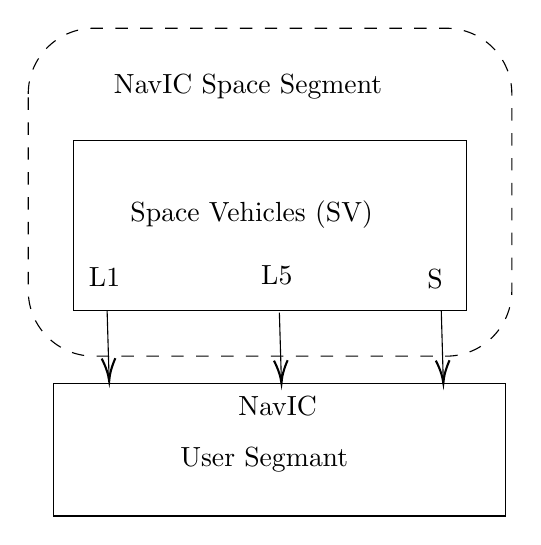
\begin{tikzpicture}[x=0.75pt,y=0.75pt,yscale=-1,xscale=1]
%uncomment if require: \path (0,406); %set diagram left start at 0, and has height of 406

%Shape: Rectangle [id:dp7411978076301706] 
\draw   (254,164) -- (443,164) -- (443,246) -- (254,246) -- cycle ;
%Straight Lines [id:da11098118487919195] 
\draw    (270,246) -- (270.94,278) ;
\draw [shift={(271,280)}, rotate = 268.32] [color={rgb, 255:red, 0; green, 0; blue, 0 }  ][line width=0.75]    (10.93,-3.29) .. controls (6.95,-1.4) and (3.31,-0.3) .. (0,0) .. controls (3.31,0.3) and (6.95,1.4) .. (10.93,3.29)   ;
%Shape: Rectangle [id:dp29610782491063636] 
\draw   (244,281) -- (462,281) -- (462,345) -- (244,345) -- cycle ;
%Straight Lines [id:da1330694648577655] 
\draw    (353,247) -- (353.94,279) ;
\draw [shift={(354,281)}, rotate = 268.32] [color={rgb, 255:red, 0; green, 0; blue, 0 }  ][line width=0.75]    (10.93,-3.29) .. controls (6.95,-1.4) and (3.31,-0.3) .. (0,0) .. controls (3.31,0.3) and (6.95,1.4) .. (10.93,3.29)   ;
%Straight Lines [id:da06268750746850027] 
\draw    (431,246) -- (431.94,279) ;
\draw [shift={(432,281)}, rotate = 268.36] [color={rgb, 255:red, 0; green, 0; blue, 0 }  ][line width=0.75]    (10.93,-3.29) .. controls (6.95,-1.4) and (3.31,-0.3) .. (0,0) .. controls (3.31,0.3) and (6.95,1.4) .. (10.93,3.29)   ;
%Rounded Rect [id:dp5981425610685245] 
\draw  [dash pattern={on 4.5pt off 4.5pt}] (232,141.6) .. controls (232,124.15) and (246.15,110) .. (263.6,110) -- (433.4,110) .. controls (450.85,110) and (465,124.15) .. (465,141.6) -- (465,236.4) .. controls (465,253.85) and (450.85,268) .. (433.4,268) -- (263.6,268) .. controls (246.15,268) and (232,253.85) .. (232,236.4) -- cycle ;

% Text Node
\draw (272,131) node [anchor=north west][inner sep=0.75pt]   [align=left] {NavIC Space Segment};
% Text Node
\draw (280,192) node [anchor=north west][inner sep=0.75pt]   [align=left] {Space Vehicles (SV)};
% Text Node
\draw (260,224) node [anchor=north west][inner sep=0.75pt]   [align=left] {L1};
% Text Node
\draw (343,223) node [anchor=north west][inner sep=0.75pt]   [align=left] {L5};
% Text Node
\draw (423,225) node [anchor=north west][inner sep=0.75pt]   [align=left] {S};
% Text Node
\draw (332,286) node [anchor=north west][inner sep=0.75pt]   [align=left] {NavIC};
% Text Node
\draw (304,311) node [anchor=north west][inner sep=0.75pt]   [align=left] {User Segmant};

\end{tikzpicture}

	\caption{the navic bands segment blocks}
	\label{figs:bandsfig}
	\end{figure}

The Figure\ref{figs:bandsfig} above specifies the radio frequency interface between space and user segments.

The NavIC will provide basically two types of services:
	\begin{enumerate}
	\item Standard Positioning Service (SPS)
	\item Restricted Service (RS)
	\end{enumerate}

		

\subsection{Standard Positioning Service (SPS):}
	It is available to all civilian users free of charge and provides positioning, navigation, and timing information with a moderate level of accuracy. The SPS signals in NavIC primarily operate in the L5 frequency band\ref{table:bands}.
\subsection{Restricted Service (RS):}
The RS is intended for authorized users and offers enhanced accuracy, integrity, and availability compared to the SPS signals. The RS signals in NavIC operate in both the L5 and S bands\ref{table:bands}.	

	
Both services will be carried on L5\ref{figure:bandsfig} and S band. The navigation signals would be transmitted in the S-band frequency and broadcast through a phased array antenna to keep required coverage and signal strength.
\\
\\
navic operated only in the L5-band and S-band frequencies. This was because India hadn't received the International Telecommunication Union authorisation for using the L1 and L2 frequency bands, which are widely used worldwide for navigation services.
\\
\\
Now that L1 band is available on the NVS-01 satellite(and will be available on subsequent NVS satellites), it is an interoperable frequency and can be used across all chipsets(of mobile devices), provided they use our signal architecture
\\
\\
All NavIC satellites transmit navigation signals in two or more frequency bands as in the table\ref{table:bands}. These signals contain ranging codes that allow receivers to compute their travelling time from satellite to receiver, along with navigation data, in order to know the satellite’s position at any time. 
%\end{document}
